% libre-compendium
%
% Copyright (C) 2026 Richard Qin
%
% This document is dual-licensed under either:
% - GNU Free Documentation License, Version 1.3 or any later version
%   published by the Free Software Foundation; with no Invariant Sections,
%   no Front-Cover Texts, and no Back-Cover Texts (see COPYING.DOC); or
% - Creative Commons Attribution-ShareAlike 4.0 International License
%   (see LICENSE-CC-BY-SA-4.0).

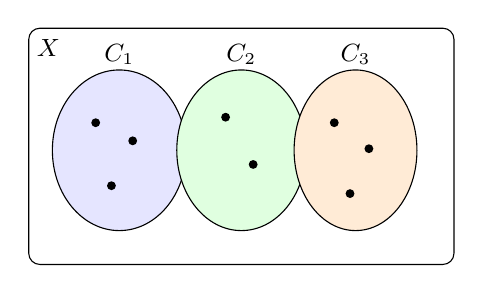
\begin{tikzpicture}[every node/.style={font=\small}]
\draw[rounded corners] (-2.6,-1.45) rectangle (2.8,1.55);
\node at (-2.35,1.3) {$X$};
\draw[fill=blue!10] (-1.45,0) ellipse (.85 and 1.02);
\draw[fill=green!12] (.1,0) ellipse (.82 and 1.02);
\draw[fill=orange!16] (1.55,0) ellipse (.78 and 1.02);
\node at (-1.45,1.22) {$C_1$};
\node at (.1,1.22) {$C_2$};
\node at (1.55,1.22) {$C_3$};
\foreach \p in {(-1.75,.35),(-1.28,.12),(-1.55,-.45),(-.1,.42),(.25,-.18),(1.28,.35),(1.72,.02),(1.48,-.55)}
  \fill \p circle (1.6pt);
\end{tikzpicture}
